\documentclass[a4paper, titlepage]{report}

\usepackage[T1]{fontenc}
\usepackage[spanish,activeacute]{babel}
\usepackage{lmodern}
\usepackage{graphicx}
\usepackage{caption,subcaption}
\usepackage{hyperref, url}

\usepackage[left=3cm,right=3cm,top=3cm,bottom=3cm]{geometry}

\title{
	\textsc{\Large{}\raggedleft{Instalación y Reemplazo de Componentes Internos}}\\
		 \vspace{18pt}
		\fontsize{40}{40}{\textbf{\texttt{LC-3}}}\\
		\Huge\textbf{\textit{Un lenguaje de bajo nivel}}
\vspace{-10pt}
}
\author{\Large{}Ariel Leonardo Fideleff}
\date{junio de 2022}

\begin{document}
	\pagenumbering{gobble}
	\maketitle
	
	\pagenumbering{arabic}
	\thispagestyle{plain}
	\tableofcontents
	
	\chapter{Introducción}
	
	\section{¡Bienvenido al bajo nivel!}
	
	\textit{¡Bienvenido al bajo nivel!}... pero paremos un segundo, ¿qué es el \textit{bajo nivel}? ¿De qué estamos hablando? Si hay un bajo nivel, también debe haber un \textit{alto nivel}, no? ¿Cómo tiene que ver todo esto con la programación?
	
	La verdad es que si bien podríamos estar ya mismo empezando a explicar un programa de ejemplo en \texttt{LC-3}, hay varios conceptos que probablemente tengamos que aclarar sobre el funcionamiento de las computadoras y algo de terminología.
	
	Ya sabemos... probablemente piensan que es aburrido. Pero creemos que si entienden algunos de estos conceptos, puedan también comprender el motivo de las limitaciones y desafíos que conlleva programar con lenguajes de bajo nivel, y del proceso lógico que lleva hacer programas en, concretamente, \texttt{LC-3}. 
	
	\section{Desde el \textit{hardware}}
	
	¿Alguna vez se preguntaron cómo un procesador formado por millones diminutos transistores de silicio es capaz de correr el juego que tanto les gusta? Si alguno se quedó en la parte de \textit{millones de transistores}, simplemente vean la imagen en la figura \ref{fig:die-img} que muestra la estructura interna de un procesador moderno.
	
	\begin{figure}[h]
		\centering
		\captionsetup{justification=centering}
		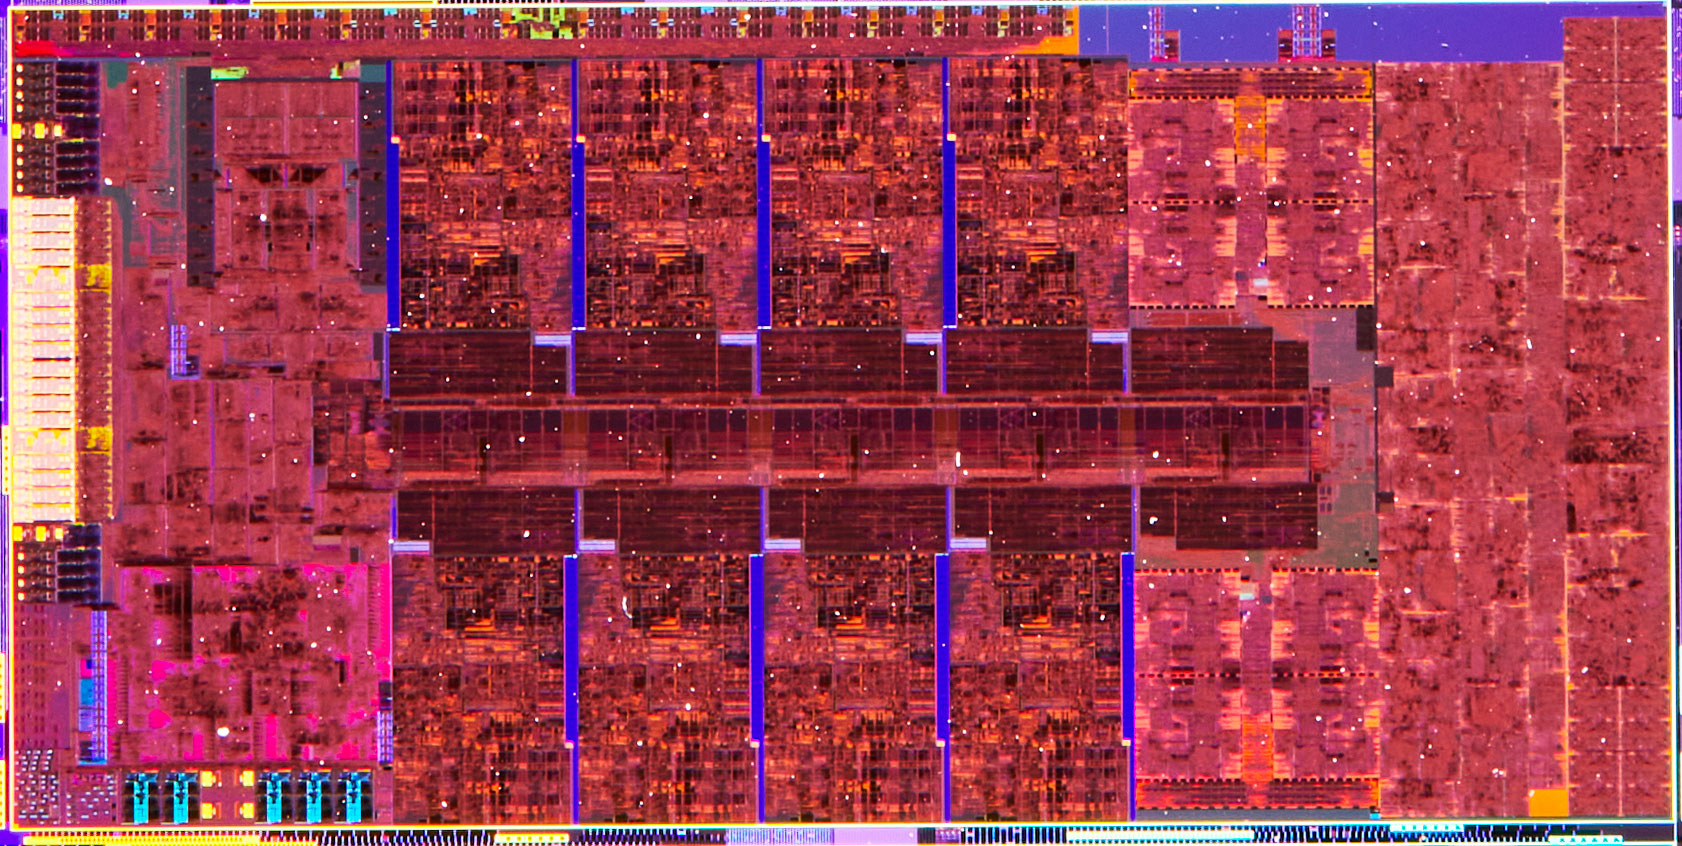
\includegraphics[width=.6\linewidth]{i9-die.jpg}
		\caption{Los millones de transistores que componen un procesador moderno, en este caso el Intel Core i9-12900K}
		\label{fig:die-img}
	\end{figure}

	No se fijen tanto en los colores, su propósito es fundamentalmente distinguir la densidad de transistores en un área determinada.
	
	A lo que apuntamos es que se empiecen a preguntar sobre todo el proceso que conlleva partir desde pulsos eléctricos, a los usos que le damos en el día a día a las computadoras (ya sea en el formato de torre de escritorio, una notebook, o un celular).
	
	Con esto en cuenta, es desde esa placa de silicio que parte todo. Todos los programas que forman el \textit{software} deben de correr en un \textit{hardware} que sea capaz de soportarlos. Y un procesador es \textit{literalmente} una parte central en un sistema de computadora\footnote{Lo entienden? CPU? \textbf{Central} Processing Unit? sigh...}.
	
	Nuestra tarea como programadores de bajo nivel es tener algunas nociones sobre el funcionamiento del hardware, con el fin de luego hacer uso de ese conocimiento, para poder confeccionar software que sea capaz de transmitirle correctamente las instrucciones necesarias para ejecutar las tareas que queramos realizar. 
	
	\section{El \texttt{ISA} y elementos de una computadora}
	
	Ya se van a dar cuenta que una de las cosas que más les gusta a los informáticos es ponerle abreviaturas a todas las cosas, más aún si nos referimos a cosas complejas con nombres largos y difíciles de recordar. Sin embargo, siempre traten de entender al menos qué es de lo que están hablando, antes que usar las abreviaturas por el resto de su vida.
	
	\subsection{El set de instrucciones}
	
	Cuando hablamos de procesadores, si bien, por ejemplo, te pueden vender la cantidad de núcleos que tienen, a nosotros nos interesa más saber que un procesador maneja tareas tales como el manejo de operaciones lógicas y matemáticas, como también el manejo de la entrada y la salida de información (conocida típicamente como \texttt{I/O}, de \textit{Input/Output} en inglés).
	
	Estas tareas son posibles a partir del \textbf{set de instrucciones} que el procesador es capaz de entender y llevar a cabo. \\
	
	Una de las cosas más difíciles al enseñar programación, es transmitir cómo uno debe desglosar en pequeñas subtareas, aquello que alguien normalmente hace intuitivamente en una hoja de papel. Por ejemplo, si nos dicen de hacer un programa en \texttt{C} para contar la cantidad de números impares en un arreglo de números, hay que pensar en cada uno de los pasos que hacemos si nos dieran el mismo problema para hacer con papel y lápiz. Así nos daremos cuenta que en nuestra cabeza, rápidamente \textit{iteramos} por cada uno de los números de la lista mientras los leemos, verificando en cada caso la condición pedida, y luego transmitimos un resultado, ya sea de forma escrita o hablada.
	
	Por lo tanto, a la hora de diseñar un procesador, el objetivo es incluir un conjunto de tareas o \textit{instrucciones} elementales, que combinadas brinden la flexibilidad necesaria para realizar cualquier tarea que queramos que una computadora lleve a cabo.
	
	Así, el \textit{set de instrucciones} de un procesador abarca las distintas instrucciones que es capaz de comprender, y que están resueltas a nivel del hardware. Estas operaciones, como dijimos, se relacionan con operaciones matemáticas (suma, multiplicación), como también con I/O (lectura y escritura en memoria, acceso a registros).
	
	\subsection{¿Y la definición?}
	
	De todas formas, probablemente habrán notado que todavía no definimos el significado de \texttt{ISA}, y eso que habíamos dicho que no había que abusar de las abreviaturas.
	
	El \textbf{Instruction Set Architecture} define un modelo abstracto fundamental de una computadora, y nos da la información de los elementos que tenemos a disposición como programadores para que nuestro software pueda interactuar con el hardware definido por una arquitectura. Para que quede claro, la arquitectura es, a modo general, el diseño de cómo va a funcionar la computadora: la interacción entre sus distintos componentes, las reglas que lo rigen y su implementación (es decir, cómo lo llevamos a cabo en un escenario real).
	
	En términos simples, el ISA especifica la parte de la arquitectura sobre qué es lo que se encuentra a disposición del programador para poder decirle a la computadora qué es lo que tiene que hacer. Es por esto que antes habíamos introducido el concepto del set de instrucciones, ya que es una de las partes principales del ISA. Reiteramos, es \textit{una de las partes principales}, pero esto no implica que sea todo.\\
	
	\subsection{¿Cómo nos llega la información?}
	
	Ya veremos que una de las instrucciones de \texttt{LC-3} es \texttt{ADD}, el cual uno puede asumir que sirve para sumar dos números. Ahora bien, pensá que un amigo te dice literalmente ``\textit{sumá dos números}''. Lo primero que uno responde es, ``\textit{¿qué números?}''. Entonces te apunta a una hoja de papel, desde la cual tenés que leer los números.
	
	Observar que tenemos que saber cómo manejar una hoja de papel para poder leer la información en ella. Podrá parecer trivial, pero es que intuitivamente sabemos cómo agarrar una hoja de papel, y disponerla frente a nuestros ojos para leer lo que esté allí escrito. Y una vez la tenemos frente a nuestros ojos, sabemos cómo interpretar lo que vemos de una forma que nuestro cerebro lo pueda comprender.
	
	Esto ilustra que las operaciones de por sí no son suficientes para que una computadora sepa lo que tiene qué hacer. De hecho, básicamente estaríamos ignorando completamente la definición de ``informática'', que entre tantas cosas abarca al \textit{conjunto de técnicas para el procesamiento, almacenamiento y transmisión de la información}. Necesitamos que la computadora sepa \textit{cómo leer} la información, así también \textit{cómo devolverla}. Por lo tanto, el ISA especifica también la forma en la que se ingresa y se presenta la información procesada al sistema, el I/O ya mencionado.
	
	La respuesta simple a la pregunta en el caso de una computadora es bueno, a través de \textit{pulsos eléctricos}. Pero... ¿cómo se ingresan esos pulsos eléctricos? ¿cómo se interpretan? ¿definen algún patrón? Las preguntas concretas sobre cómo implementarlo se las dejamos a los encargados de diseñar la arquitectura y el hardware, pero como programadores nos interesa la especificación de instrucciones que nos permitan leer y mostrar información, es decir, saber cómo usar las instrucciones que nos habilitan el I/O.
	
	En el caso de nuestro ejemplo, tenemos que tener las ``instrucciones'' para que nos digan cuando se quiere, por ejemplo, leer de un papel, y que sepamos hacerlo.
	
	\subsection{¿Cómo guardamos la información?}
	
	Una vez que pudimos leer la información, debemos de tenerla guardada en algún lugar para poder operar con ella. Esto introduce otro componente importante de una computadora, la \textbf{memoria}.
	
	En nuestro ejemplo nos dan una hoja de papel donde podemos decir que ``están almacenados'' los números, así que lo podemos considerar como un ejemplo de memoria, no? No hay que confundir la memoria con \textit{medios de almacenamiento}. De ahora en más, cuando hablemos de memoria, siempre haremos referencia a sistemas o dispositivos que nos permitan almacenar información \textbf{para su uso inmediato}.
	
	Mírenlo de esta forma: es más rápido sumar dos números cuando los tenemos ya en nuestra cabeza, que si estamos constantemente leyéndolos del papel. La memoria en este caso es nuestra capacidad de recordar los números con los que operamos, y el papel es un medio de almacenamiento que nos permite resguardar los números a largo plazo. Análogamente, esto se relaciona en cómo es más rápido leer de la memoria RAM, que de un medio de almacenamiento como un disco duro HDD o hasta un disco de estado sólido SSD.\\
	
	Dicho esto, para operar con los números, es necesario tener alguna forma de que los números permanezcan en nuestra cabeza, al menos de forma temporal. Si queremos hacer $2+2$, tenemos que acordarnos, por más que sea por fracciones de segundo, de los dos números, para saber e informar que el resultado de la operación es $4$. Así, es que el ISA define también cómo podemos acceder a la memoria, cómo podemos operar con ella, y las instrucciones relacionadas.\\
	
	En las computadoras hay distintos tipos de memoria que ocupan distintos lugares en una jerarquía que depende según su velocidad, aunque trataremos estas diferencias más adelante cuando definamos en detalle el ISA de \texttt{LC-3}.
	
	Nomás tengan en cuenta que cuando hablamos de ``memoria'' muchas veces no sólo nos referimos, como ya habíamos aclarado, a memorias de uso inmediato, sino concretamente a memorias volátiles (que no permiten almacenar información a largo plazo y que se borran cuando, por ejemplo, se les quita energía) a las cuales podemos acceder a sus contenidos de forma aleatoria (modificar y acceder a distintas partes de la memoria rápidamente). Hoy en día, este tipo de memorias las conocemos como \textit{memorias RAM} (Random Access Memory, en español, memorias de acceso aleatorio).
	
	Créannos que a lo largo de este texto se les va a ir aclarando de lo que estamos hablando.
	
	\subsection{¿La operación se guarda?}
	
	Entonces ya sabemos leer los números, guardarlos, hacer la operación, y devolver el resultado. ¿Nos falta algún paso más?
	
	En vez de dar una respuesta, vamos a proponer otra pregunta: ¿La operación dónde está guardada? Dicho de otra forma, ¿de dónde lee la computadora la operación?
	
	La respuesta lógica a esta pregunta es que la operación se encuentra en un programa, y ese programa necesariamente tiene que estar en la memoria. Al fin y al cabo, el programa es con el cual estamos haciendo operaciones en el uso inmediato.
	
	Pero en la memoria también habíamos guardado los números una vez los habíamos leído. Esto nos lleva a la pregunta: ¿cómo distinguimos la memoria en dónde está nuestro programa, con la memoria de la información que leímos?
	
	Tantas preguntas y pocas respuestas...\\
	
	Cuando queremos acordarnos de alguna cosa, generalmente sólo ``lo pensamos'' y con suerte nos acordamos y podemos utilizar la información obtenida. Si bien los científicos podrán no saber con exactitud todavía cómo funciona este proceso, mientras tanto tenemos que tener alguna forma de diseñar una memoria que nos permita acceder a los distintos fragmentos de información que contiene de una forma ordenada. Es por esto que la memoria tiene \textbf{direcciones de memoria}, que funcionan como identificadores para cada uno de los sectores de la memoria que podemos acceder de forma independiente según nuestras necesidades. 
	
	
	
	%Es por esto que el ISA, además del set de instrucciones, define lo que se conocen como \textbf{addressing modes}, que en español conocemos como \textit{modos de direccionamiento}.
	
	%A modo práctico, incluye las distintas formas en las que podemos indicar dónde se encuentra la información, cuando ejecutamos una instrucción. Veremos aquellos que \texttt{LC-3} tiene a medida que vayamos introduciendo las distintas instrucciones que los usan.\\
	
	
	\subsection{Pasando en limpio}
	
	% i/o
	% data types
	% memory

	\section{Una vez más, ¿qué significa \textit{alto} y \textit{bajo} nivel?}
	
	Para que se sientan más familiares con lo que vamos a hablando, vamos a estar comparando o relacionando lo que expliquemos con el lenguaje \texttt{C}, el cual ya probablemente conocen por su trayecto en la escuela. Al fin y al cabo, es más sencillo partir desde lo que ya saben, que explicar todo desde cero.
	
	Cuando 
	
	\section{Felicitaciones, se ahorró más de 150 páginas de lectura}

	La realidad es que mucha información se perdió entre medio, pero nos enfocamos en lo necesario para continuar con el próximo capítulo.
	
	\chapter{Bibliografía} % extender y armar bien posta
	
	\begin{itemize}
		\item \url{https://www.techpowerup.com/review/intel-core-i9-12900k-alder-lake-12th-gen/2.html}
		\item \url{https://www.gamersnexus.net/guides/833-reading-a-cpu-die}
		\item Introduction to Computer Systems, Patt \& Patel % extender y armar bien
	\end{itemize}
	
\end{document}